\documentclass[10pt]{beamer}
\usepackage[russian]{babel}
\usepackage[utf8]{inputenc}
\usepackage[T2A]{fontenc}
\inputencoding{utf8}
\usepackage{amssymb,amsfonts,amsmath,mathtext,amsthm,mathtools}
\usepackage{float}
\usepackage[dvips]{graphicx}
\usepackage[unicode, pdfborder = {0 0 0}, colorlinks, linkcolor = black]{hyperref}
\usepackage{sansmathaccent}
\pdfmapfile{+sansmathaccent.map}
\usetheme{Frankfurt}
% \usecolortheme{seahorse}
\title{Восстановление циклически смазанных изображений с вырожденным смазом}
\author[Ковалев~Н.~Е.]{Ковалев~Никита~Евгеньевич\\научный руководитель -\\доц., к.ф.-м.н., Козак~Анатолий~Всеволодович}
\institute[ЮФУ, ИММиКН]{Южный федеральный университет\\ Институт математики, механики и компьютерных наук им. И.И. Воровича}
\date{Ростов-на-Дону, 2018}


\DeclarePairedDelimiter\ceil{\lceil}{\rceil}
\DeclarePairedDelimiter\floor{\lfloor}{\rfloor}

\setcounter{tocdepth}{5}
\setcounter{secnumdepth}{5}

\newcounter{qcounter}


\makeatletter
\defbeamertemplate*{footline}{my theme}{
	\leavevmode%
	\hbox{%
	\begin{beamercolorbox}[wd=.3\paperwidth,ht=2.25ex,dp=1ex,center]{author in head/foot}%
		\usebeamerfont{author in head/foot}%
		\insertshortauthor~~\beamer@ifempty{\insertshortinstitute}{}{(\insertshortinstitute)}
	\end{beamercolorbox}%
	\begin{beamercolorbox}[wd=.7\paperwidth,ht=2.25ex,dp=1ex,center]{title in head/foot}%
		\usebeamerfont{title in head/foot}\inserttitle
	\end{beamercolorbox}}%
}
\makeatother


\setbeamertemplate{caption}[numbered]


\begin{document}

\begin{frame}
\maketitle
\end{frame}


\section{Цели работы}
\begin{frame}
\begin{block}{\LARGE{Цели работы}}
\begin{list}{\arabic{qcounter})~}{\usecounter{qcounter}}
\item Исследовать матрицу смаза, ее свойства
\item Изучить возможность упрощения задачи восстановления
\item Найти общий способ восстановления изображений с вырожденным смазом
\end{list}
\end{block}
\end{frame}



\section{Вспомогательные утверждения}
\begin{frame}
\begin{block}{\emph{Матрица горизонтального циклического смаза} (далее - \emph{матрица смаза}) на $k$ пикселей}
    $$
    C(n, k) = \frac{1}{k}\begin{pmatrix}
          \overbrace{1 \hspace*{2mm} \ldots \hspace*{2mm} 1 \hspace*{2mm} 1}^{k} \hspace*{2mm} 0 \hspace*{2mm} \ldots \hspace*{2mm} 0 \\
          0 \hspace*{2mm} 1 \hspace*{2mm} \ldots \hspace*{2mm} 1 \hspace*{2mm} 1 \hspace*{2mm} \ldots \hspace*{2mm} 0 \\
          \ldots \hspace*{2mm} \ddots \hspace*{2mm} \ldots \hspace*{2mm} \ddots \hspace*{2mm} \ldots \\
          1 \hspace*{2mm} \ldots \hspace*{2mm} 0 \hspace*{2mm} 1 \hspace*{2mm} 1 \hspace*{2mm} \ldots \hspace*{2mm} 1 \\
          \ldots \hspace*{2mm} \ddots \hspace*{2mm} \ldots \hspace*{2mm} \ddots \hspace*{2mm} \ldots\\
          \underbrace{1 \hspace*{2mm} \ldots \hspace*{2mm} 1}_{k-1} \hspace*{2mm} 0 \hspace*{2mm} 0 \hspace*{2mm} \ldots \hspace*{2mm} 1
        \end{pmatrix}
    $$
\end{block}
\begin{block}{\emph{Горизонтальный циклический смаз} (далее - \emph{смаз})}
Умножение изображения на соответствующую матрицу смаза справа есть смаз.
\end{block}
\begin{block}{Утверждение.}
 Матрица смаза всегда представима в виде $FDF^{-1}$, где $D$ - диагональная.
\end{block}

\end{frame}


\section[Метод разбиения]{Метод предобработки в случае большого числа смаза}
\begin{frame}
\begin{block}{Подход}
Главная идея метода - разбить задачу вырожденного смаза на несколько подзадач с невырожденным смазом.
Пусть $n$ - ширина изображения в пикселах, $k$ - число смаза и $d =$ НОД$(n, k)$. Тогда, если $d > 1$, разобьем изображение на $d$ частей, взяв из $d$ подряд идущих колонок ровно одну в каждую часть.
\end{block}

\begin{block}{}
 \begin{figure}[H]
            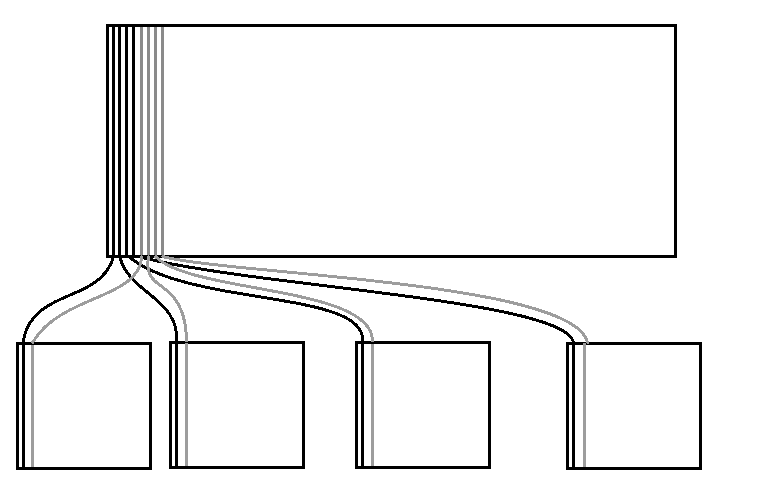
\includegraphics[scale=0.2]{fig1.png}
            \label{Pic1}
            \caption[Разбиение изображения на несколько подизображений]{Разбиение изображения на несколько подизображений}
        \end{figure}
\end{block}

\end{frame}

\begin{frame}

\begin{block}{Причина смаза на $d$ пикселей в результате}


\begin{equation}\label{1}
\frac{x_1 + x_2 + ... + x_k}{k} = \frac{\frac{x_1 + ... + x_d}{d} + \frac{x_{d+1} + ... + x_{2d}}{d} + ...}{p}, p = \frac{k}{d}
\end{equation}
\begin{equation}\label{2}
\frac{x_2 + x_3 + ... + x_{k+1}}{k} = \frac{\frac{x_2 + ... + x_{d+1}}{d} + \frac{x_{d+2} + ... + x_{2d+1}}{d} + ...}{p}
\end{equation}

Восстанавливаем каждое подизображение с числом смаза $p$. Получим, что пиксели восстановленного изображения (собранного из восстановленных кусков по тому же принципу разбиения) имеют вид:


{\Large$\frac{x_1 + x_2 + ... + x_d}{d}$} - первый пиксель, полученный из пикселя (1).


{\Large$\frac{x_2 + x_3 + ... + x_{d+1}}{d}$} - первый пиксель, полученный из пикселя (2).


Видно, что в итоге соседние пиксели это среднее арифметическое $d$ соседних пикселей исходного, сдвинутых на 1 при переходе к следующему, то есть смаз с числом смаза $d$

\end{block}

\end{frame}

\begin{frame}
\begin{block}{Пример 1}
\begin{minipage}{50mm}
    \begin{figure}[H]
            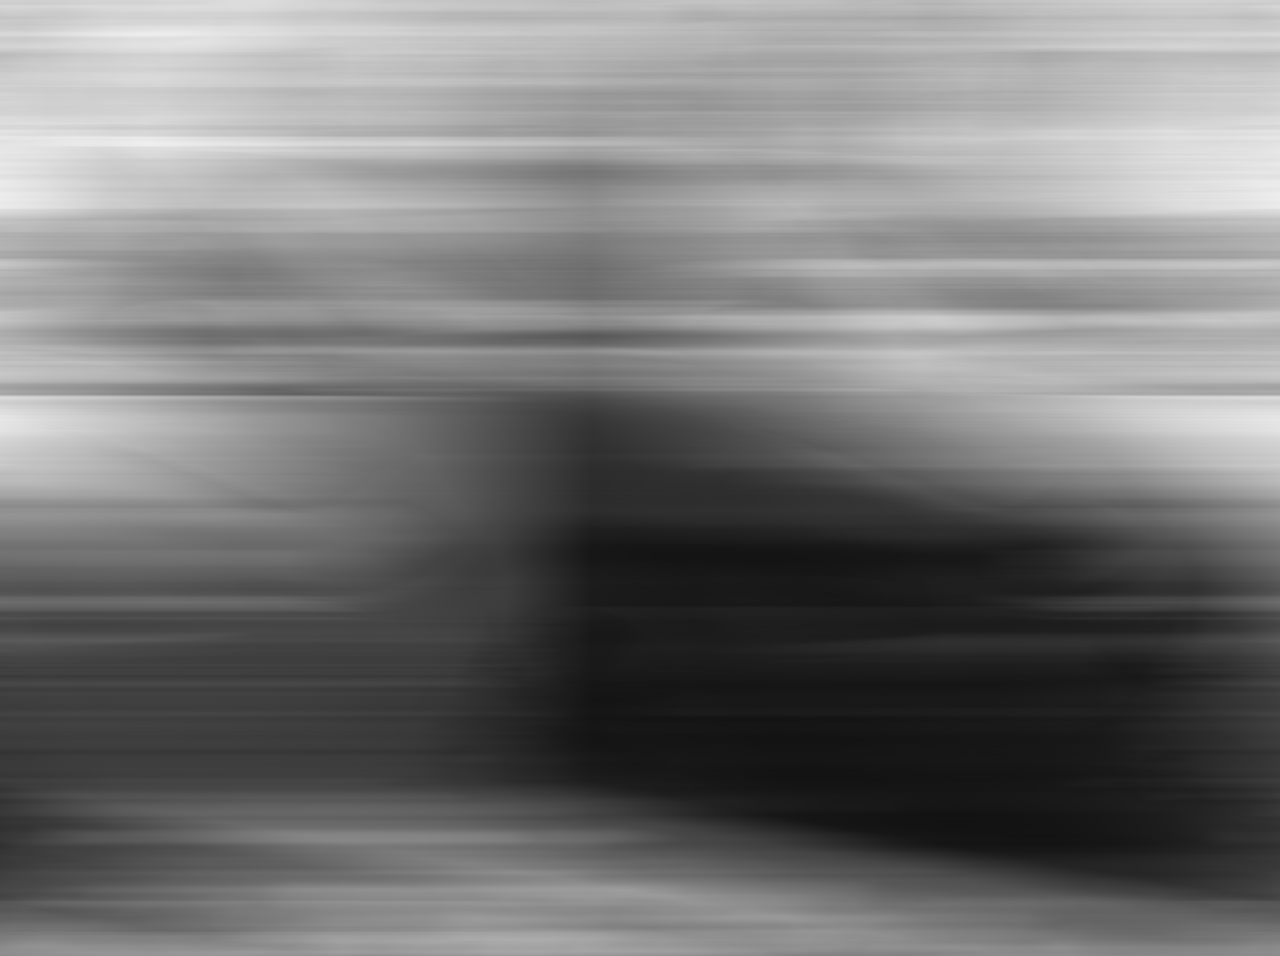
\includegraphics[scale=0.11]{G:/Study/tex_diploma/Pictures/fig3.png}
            \label{Fig3}
            \caption[Смаз при $k$ = 592]{Смаз при $k$ = 592}
        \end{figure}
\end{minipage}
\hspace{5mm}
\begin{minipage}{50mm}
  \begin{figure}[H]
            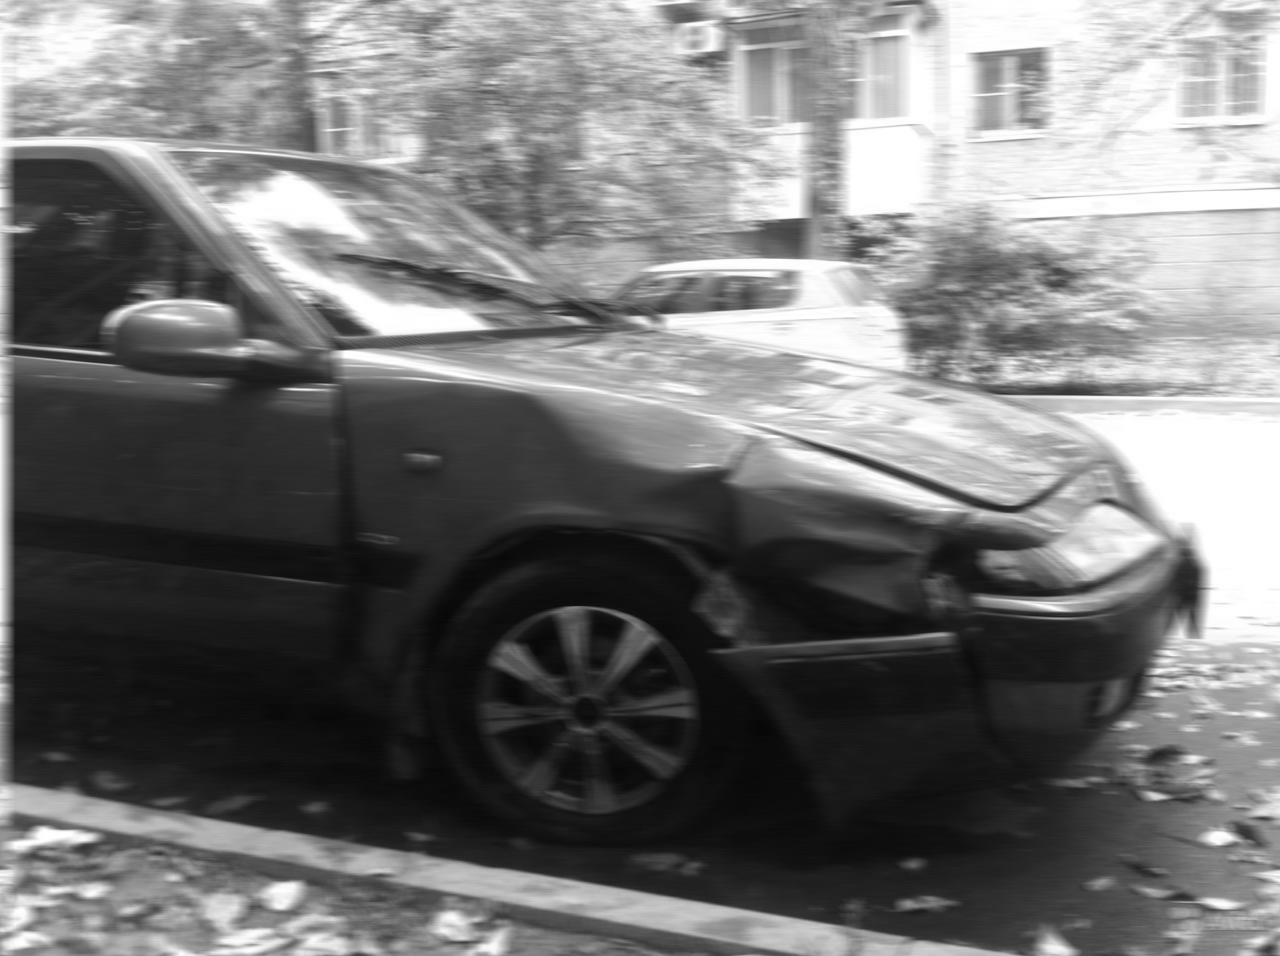
\includegraphics[scale=0.11]{G:/Study/tex_diploma/Pictures/fig4.png}
            \label{Fig4}
            \caption[Улучшенное фото]{Улучшенное фото}
        \end{figure}
\end{minipage}
\hfill
\end{block}

\end{frame}



\section[Метод минимизации]{Метод минимизации погрешности}
\begin{frame}
\begin{block}{Описание проблемы}
Матрица $C$ в общем случае может быть необратима. Тогда для восстановления необходимо построить приближение $\tilde{C}$ таким образом, что $C\tilde{C}$ приближает единичную матрицу там, где это возможно.


Особенность задачи --- наличие погрешности (округления и вычислений), возникающей по причине оцифровке изображений и вследствие плохой обусловленности матрицы смаза.
\end{block}

\begin{block}{}
Учитывая все вышесказанное, а также свойство матрицы $C$ о представлении в диагональном виде, предлагается строить матрицу $\tilde{C}$, используя ее разложение и проебразуя собственные числа, лежащие на диагонали получившейся матрицы.
\end{block}

\end{frame}


\begin{frame}

\begin{block}{О преобразованиях}
Будем применять к собственным числам линейные преобразования:
    \begin{list}{\arabic{qcounter})~}{\usecounter{qcounter}}
        \item Необратимость будем устранять заменой нулевых собственных чисел на некоторые числа с фиксированным модулем (модуль, так как собственные числа являются комплексными);
        \item Погрешность вычислений минизируем тем же способом~-~к ненулевым собственным числам, которые сильно малы по модулю, прибавим случайное комплексное число с тем же фиксированным модулем;
        \item Кроме того, оставшиеся достаточно малые собственные числа домножим так, чтобы по модулю они были равны фиксированному числу.
    \end{list}
\end{block}

\end{frame}


\begin{frame}

\begin{block}{Поправка по умножению}
Пусть поправка по умножению $\delta_i, i = \overline{0, n-1}$, $C = FDF^{-1}$, $\tilde{C} = F\tilde{D}F^{-1}$, $\tilde{E} = D\tilde{D}$. Тогда $E = diag(\frac{d_0}{d_0\delta_0}, \frac{d_1}{d_1\delta_1}, ...)$ $=$ $diag(\delta_0^{-1}, \delta_1^{-1}, ...)$, где $d$ - вектор собственных чисел матрицы $C$.


Восстановление: $(XC)\tilde{C} = XFDF^{-1}F\tilde{D}F^{-1} = XFD\tilde{D}F^{-1} = XF\tilde{E}F^{-1}$. Пусть $R = F\tilde{E}F^{-1}$, тогда $R_{ij} = \frac{1}{n}\Sigma_{k=0}^{n-1} \delta_k^{-1} \xi^{(j-i)k}$, где $\xi = e^{\frac{2\pi}{n}}$.
\end{block}

\begin{block}{Пояснение о числах на разных диагоналях}
\begin{minipage}{50mm}
    \begin{figure}[H]
            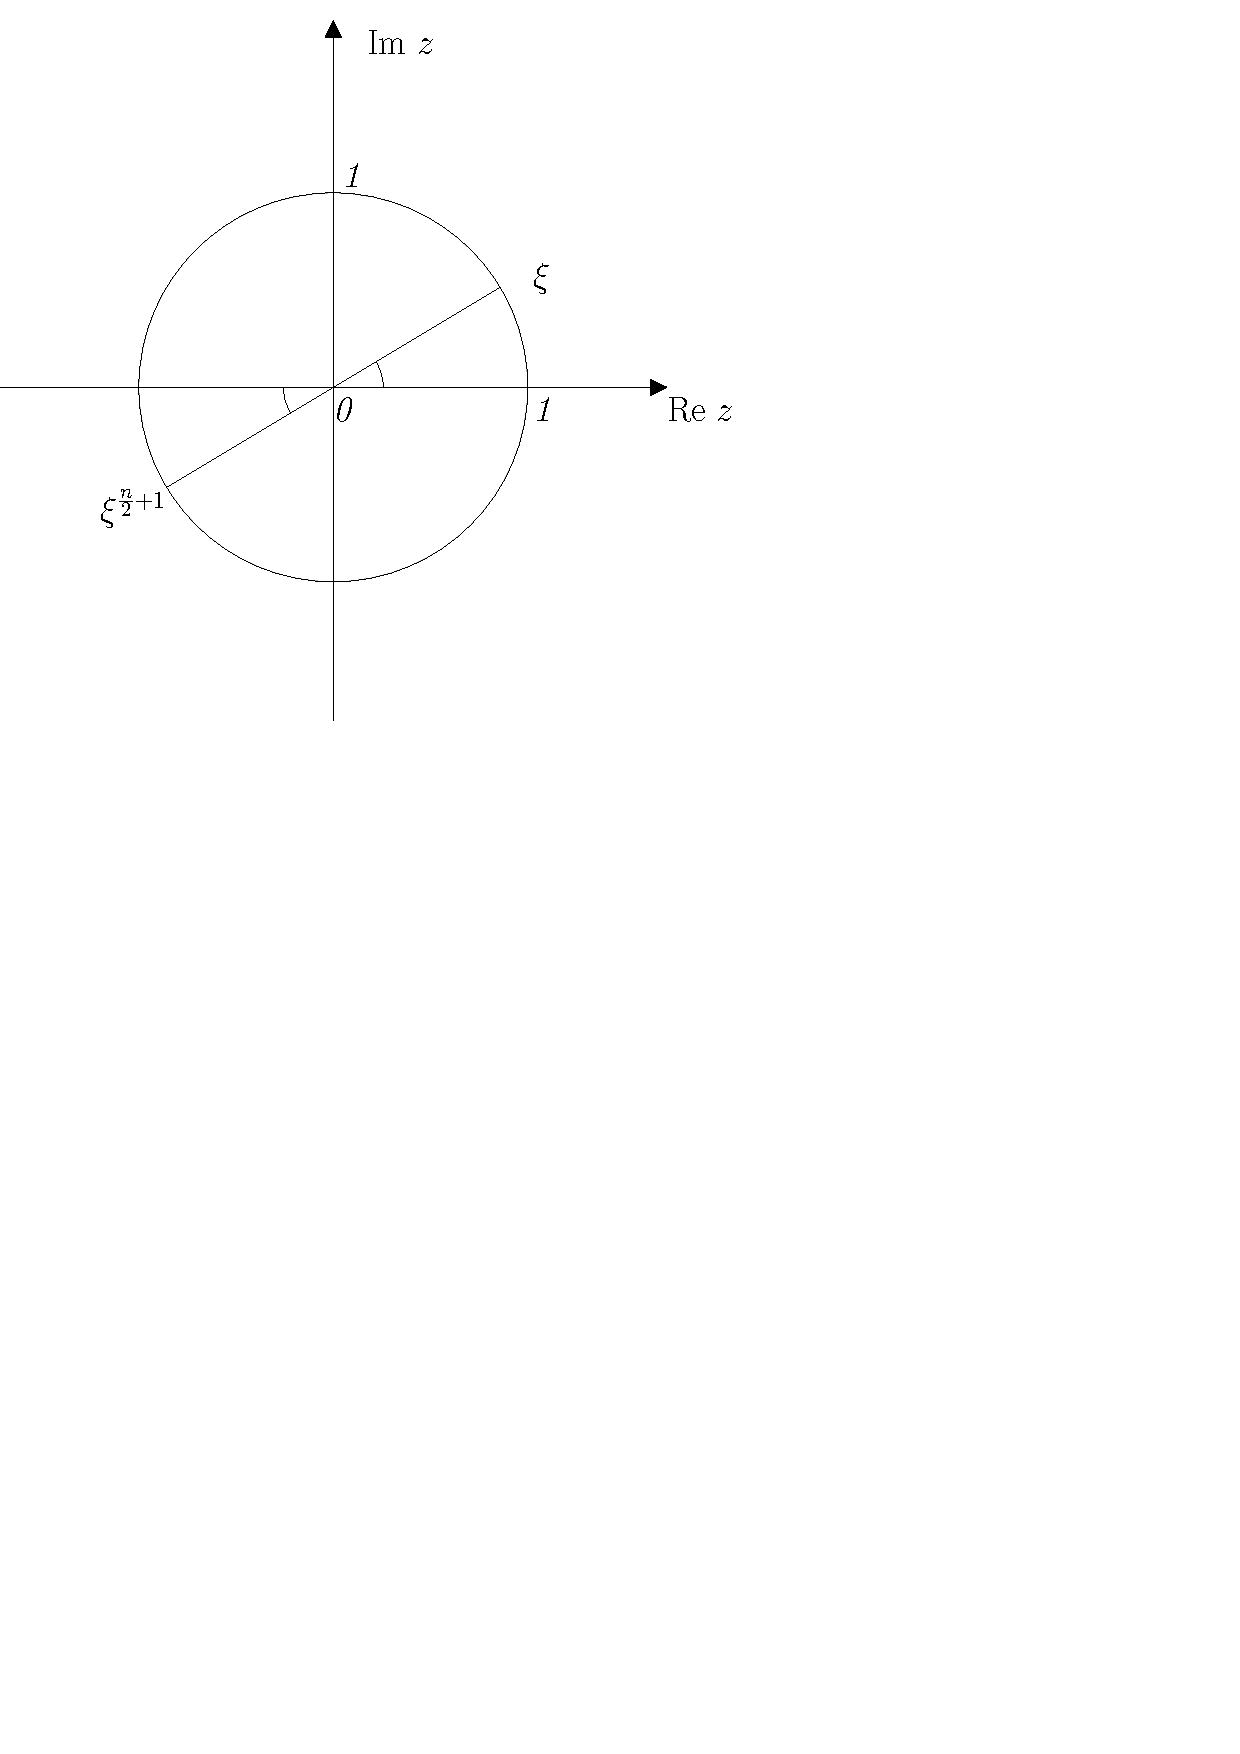
\includegraphics[scale=0.3]{G:/Study/tex_diploma/Pictures/graph1.pdf}
            \label{Graph1}
            \caption[Значения на первой диагонали после главной]{Значения на первой диагонали после главной}
        \end{figure}
\end{minipage}
\hfill
\begin{minipage}{50mm}
  \begin{figure}[H]
            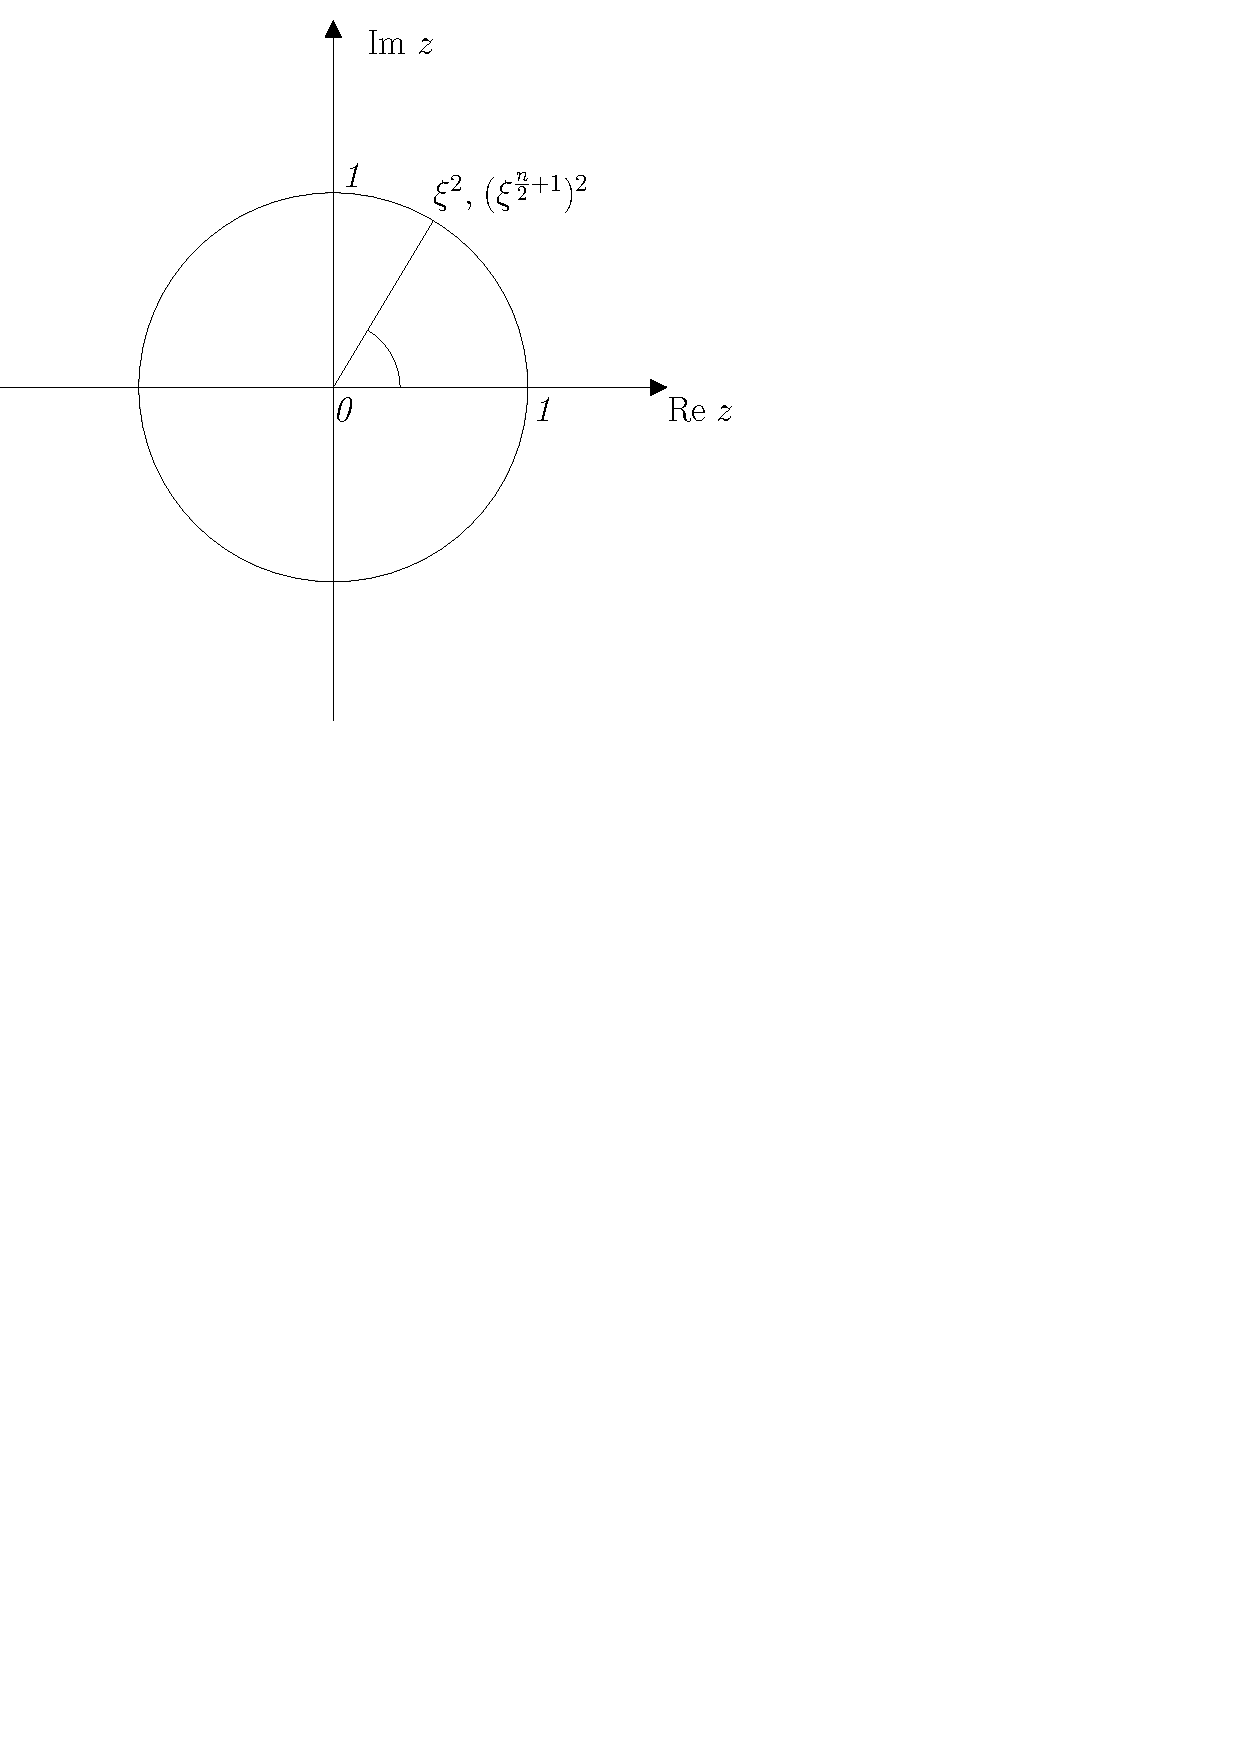
\includegraphics[scale=0.3]{G:/Study/tex_diploma/Pictures/graph2.pdf}
            \label{Graph2}
            \caption[Значения на второй диагонали после главной]{Значения на второй диагонали после главной}
        \end{figure}
\end{minipage}
\hfill
\end{block}

\end{frame}



\begin{frame}

\begin{minipage}{50mm}
    \begin{figure}[H]
            \includegraphics[scale=0.05]{G:/Study/tex_diploma/Pictures/fig9.png}
            \label{Pic9}
            \caption[Восстановление с поправкой по умножению]{Восстановление с поправкой по умножению}
        \end{figure}
\end{minipage}
\hfill
\begin{minipage}{50mm}
    \begin{figure}[H]
            \includegraphics[scale=0.05]{G:/Study/tex_diploma/Pictures/fig11.png}
            \label{Pic9}
            \caption[Восстановление без поправки]{Восстановление без поправки}
        \end{figure}
\end{minipage}
\vspace*{2mm}

\end{frame}

\begin{frame}

\begin{minipage}{100mm}
  \begin{figure}[H]
            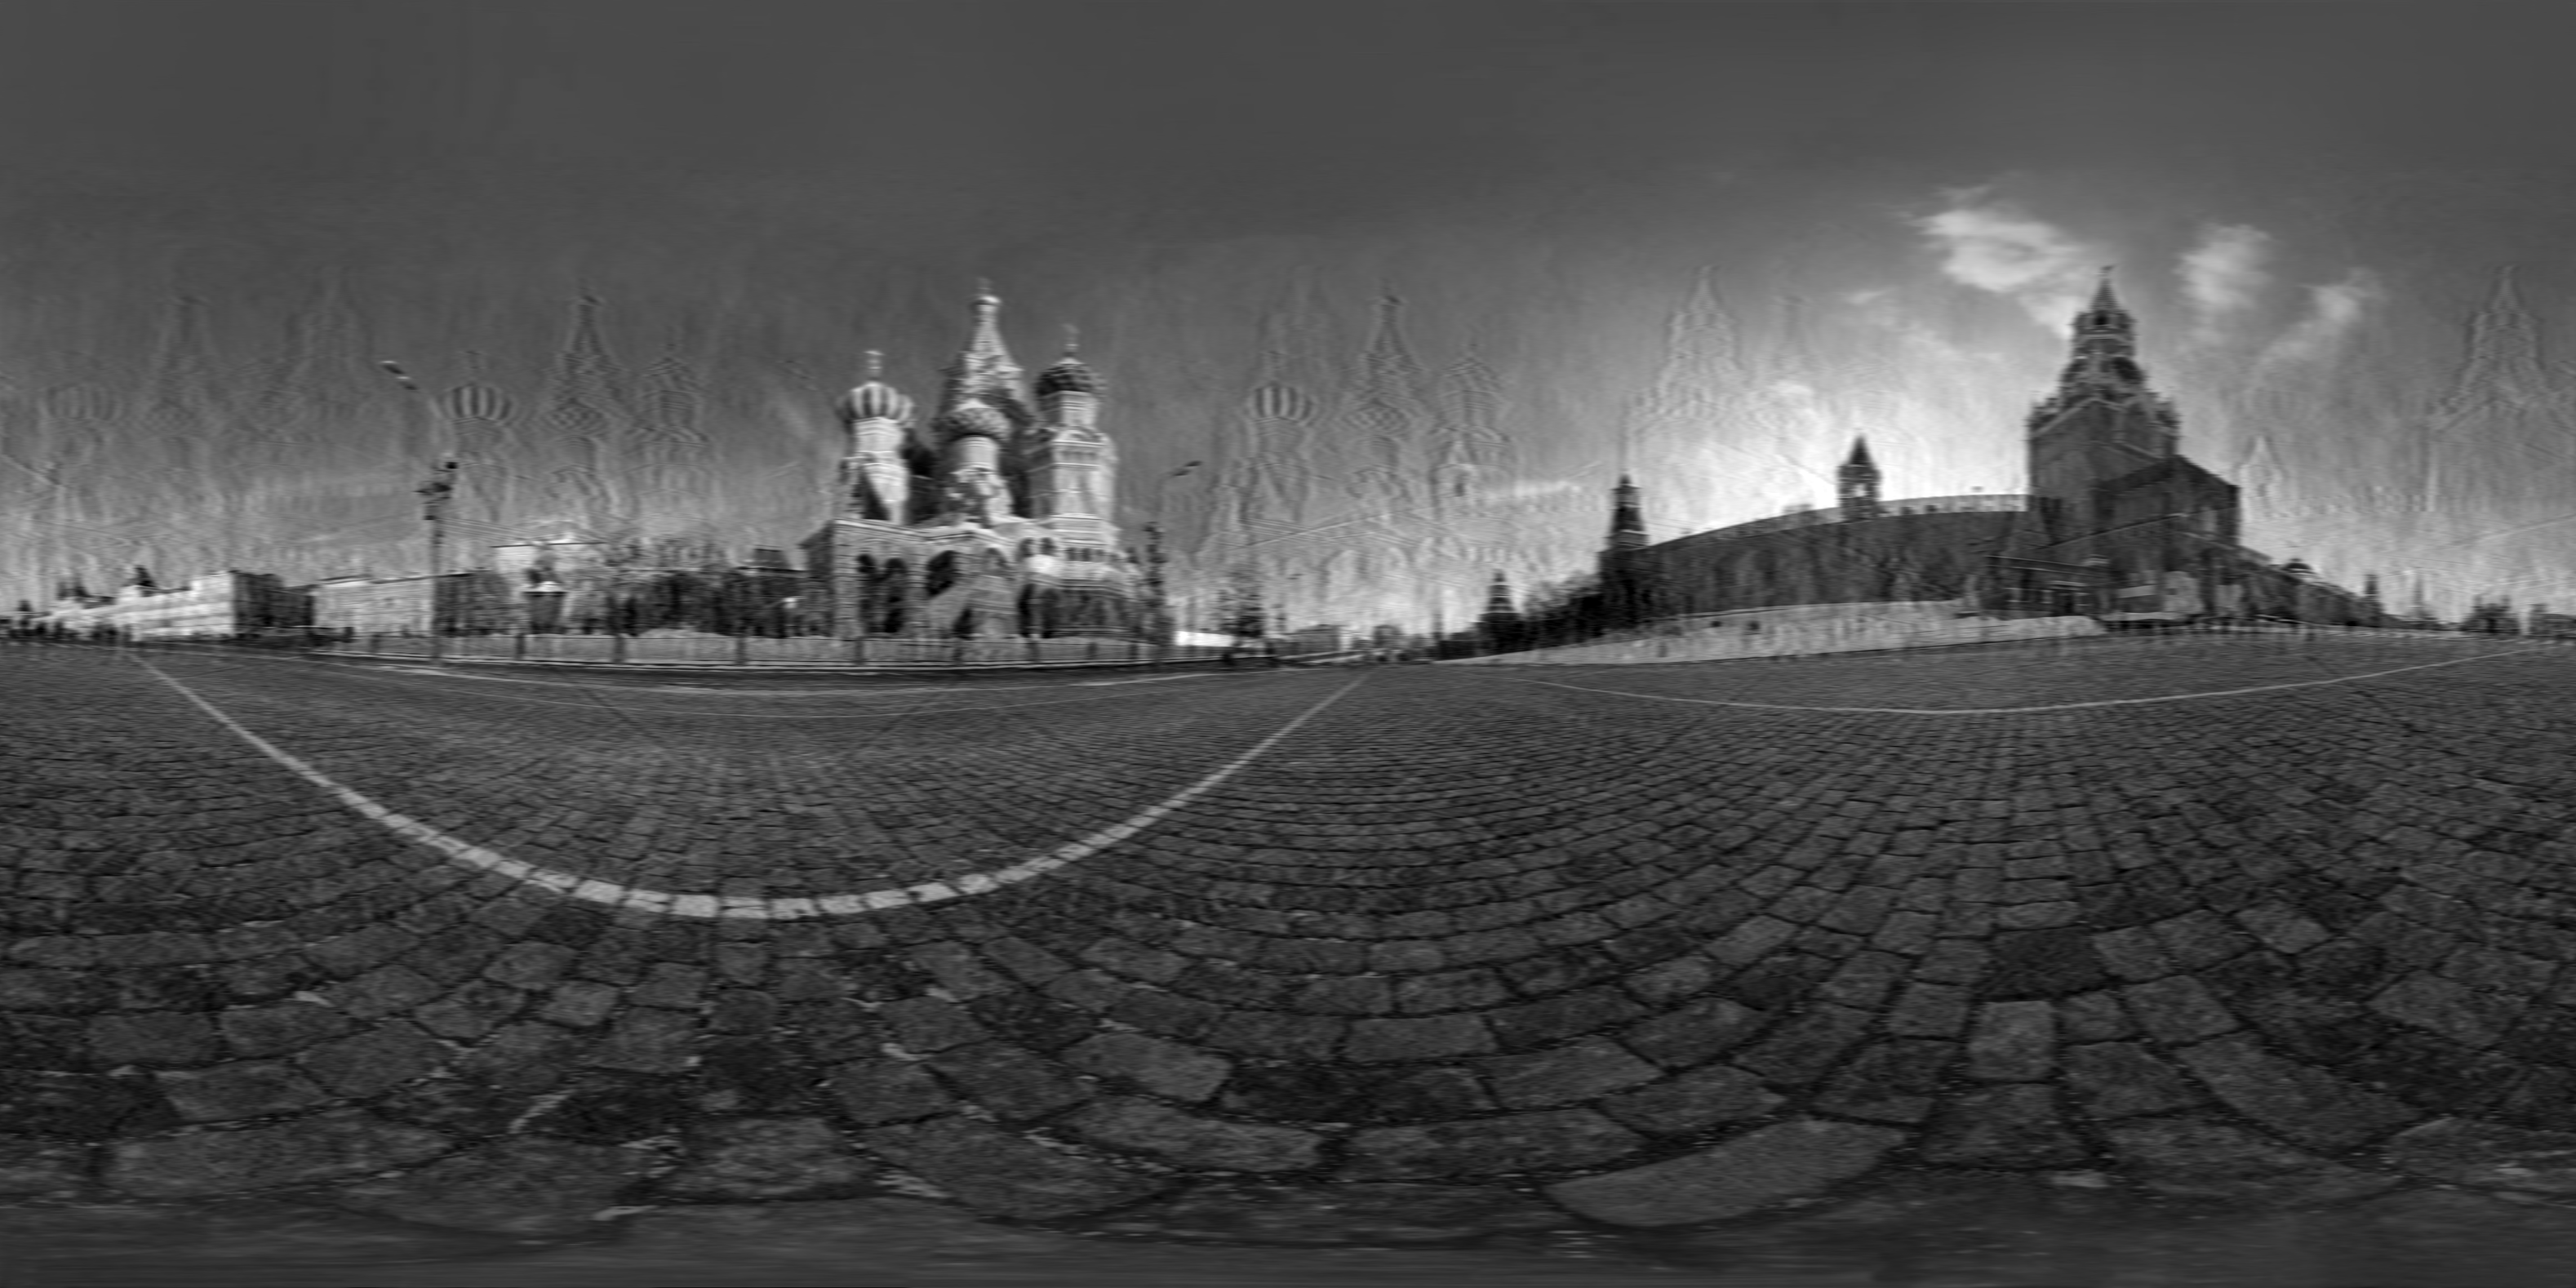
\includegraphics[scale=0.1]{G:/Study/tex_diploma/Pictures/fig10.png}
            \label{Pic10}
            \caption[Восстановление с применением поправки по сложению]{Восстановление с применением поправки по сложению}
        \end{figure}
\end{minipage}
\hfill

\end{frame}



\end{document}